\documentclass[11pt]{article}
\usepackage[margin=1in]{geometry}
\usepackage[T1]{fontenc}
\usepackage{lmodern}
\usepackage{graphicx}
\usepackage{booktabs}
\usepackage{tabularx}
\usepackage{amsmath}
\usepackage{xcolor}
\usepackage[hidelinks]{hyperref}
\usepackage{enumitem}
\setlist{nosep,leftmargin=1.4em}

\title{Verified-Answer Precision as the Acceptance Test for Speed and Quantization:\\
A Qwen3.8-Flash-Next Tool Agent for ARC-AGI-2 on Four L4 GPUs}
\author{Md.\ Hamid Hosen \and FOYSAL \and Esfer Sami\\[2pt]
\small Team Hack2Publish, ARC Prize 2026}
\date{November 2026}

\begin{document}
\maketitle

\begin{abstract}
On fixed hardware, an ARC-AGI-2 system can be made faster by compressing the model or by running more sessions at once.
We argue, and test on our own runs, that such a change should be accepted only if the precision of \emph{verified} answers does not fall: a program that reproduces every demonstration pair is the system's own unit test, and a weaker model passes that test with the wrong rule more often.
We document our submission 57851995 (public leaderboard 54.17\,\%): Qwen3.8-Flash-Next served offline on Kaggle's 4$\times$L4 machine with 4-bit routed experts, an FP8 KV cache and 3-token multi-token-prediction speculation, driving nine concurrent sessions of a Python tool agent that checks candidate programs on the training pairs.
Comparing it with a faster 3-bit build of the same agent:
(i)~on the first attempts of 6-hour runs over the 120 public evaluation tasks, train-verified programs were correct on the test 77.2\,\% of the time at W4A16 and 62.5\,\% at 3 bits (Fisher $p=0.037$); on 15 matched tasks the figures were 24/26 vs 22/28;
(ii)~11 of the 15 train-verified wrong programs we found implement a rule the demonstrations do not determine, and both W4A16 errors produced the same wrong grids as the 3-bit build;
(iii)~the 3-bit build generated 2.3$\times$ the tokens, started all 120 tasks where the W4A16 build reached 92, and won on evaluation (65.0 vs 53.75 task-normalised), yet on the 92 tasks both reached it solved fewer (57 vs 63), and on the leaderboard it scored 49.58 against our 54.17;
(iv)~a paired FP8-vs-BF16 KV test solved 13/15 tasks each while FP8 fitted 9 sessions instead of 5.
We also report a thinking-cap inversion for a dense 27B model, an evaluation-versus-leaderboard rank inversion between two public notebooks, a cross-system union oracle, and a ledger of negative results.
Our precision result independently replicates, with matched tasks and at a low-throughput operating point, an observation by another 2026 team.
\end{abstract}

\section{Introduction}
ARC-AGI measures the ability to acquire a new skill from a handful of examples \cite{chollet2019,arcagi2}. Each task shows two to five input/output grid pairs; the solver must produce the exact output grid for one or two test inputs, with two attempts each. The tasks are easy for people and hard for current AI systems, which makes the benchmark a probe of generalisation rather than of memorised knowledge \cite{arctr2025}.
The ARC Prize 2026 competition runs a submitted notebook on 240 hidden tasks within 12 hours on four 24\,GB NVIDIA L4 GPUs, without internet access.

Language models that write and test programs are the strongest approach on this hardware in 2026 \cite{greenblatt2024,pivotools2026,notnitsuj2026}. The score is roughly the product of \emph{coverage} (the share of tasks that get a full attempt) and the \emph{solve rate} of an attempt. Both draw on the same budget: compression or more concurrency raises coverage but can lower the quality of each attempt.

Our approach grew out of our own leaderboard history (Figure~\ref{fig:lb}): seven months of test-time-training reproductions stayed at or below 32.64, a dense 27B model reached 34.58, and a sparse Flash-Next agent reached 54.17. A faster 3-bit version of the same agent covered more of the evaluation set yet scored lower on the leaderboard. This paper explains why and turns it into a rule.

\paragraph{Contributions.}
\begin{enumerate}
\item \textbf{A decision rule with matched evidence.} Accept a speed or compression change only if verified-answer precision $\times$ verified answers per hour does not fall. We measure precision for W4A16 and 3-bit builds on matched tasks with confidence intervals (Section~\ref{sec:precision}), and classify every train-verified wrong program (Table~\ref{tab:fv}).
\item \textbf{A coverage-versus-precision decomposition} of two 6-hour runs: where the faster build wins (tasks the slower one never reaches) and where it loses (the tasks both reach).
\item \textbf{Three evaluation-versus-leaderboard inversions}, including one between two public notebooks run by us under equal windows, and a cap inversion for a dense 27B model.
\item \textbf{A negative-results ledger and a union oracle} that bound what complementary systems could add, and a reproducible low-throughput recipe (Section~\ref{sec:system}, Appendix~\ref{app:spec}).
\end{enumerate}

\section{Related work}
\paragraph{Test-time training.} The ARChitects \cite{architects2024,architectspoe} and NVARC \cite{nvarc2025} fine-tune a small model per task and rank sampled grids by augmentation scores; Aky\"urek et al.\ \cite{akyurek2024} studied test-time training on ARC. Our companion paper \cite{paper1} decomposes our NVARC-derived runs into generation and selection.
\paragraph{Program synthesis with verification.} Greenblatt \cite{greenblatt2024} sampled many programs and kept those that reproduce the demonstrations; Li et al.\ \cite{li2024} combined induction and transduction; SOAR \cite{soar2025} evolves programs with self-improving models; Poetiq \cite{poetiq} refines code with training-pair feedback; pivotools \cite{pivotools2026} showed that an agentic Python loop improves ARC-AGI-2 scores across models. The Duck harness \cite{duck} won ARC-AGI-3 Milestone~1 with a persistent Python tool; our agent uses Franzen's fork of it \cite{duckfork} with an ARC-AGI-2 adapter.
\paragraph{2026 Flash-Next systems on 4$\times$L4.} Several teams published writeups with the same model and hardware (Table~\ref{tab:public}). notnitsuj \cite{notnitsuj2026} reports that compression shows up as less precise verified programs rather than fewer of them, that memory sets throughput, and that aborting slow sessions costs points. Our precision result is an independent replication with a different pair of precisions (W4A16 vs 3-bit, all 512 experts, no pruning or training) and matched tasks.

\begin{table}[t]
\centering\small
\begin{tabularx}{\linewidth}{@{}lrrrX@{}}
\toprule
System (writeup) & Public LB & tok/s & Sessions & Compression; selection \\
\midrule
Yi-Chia Chen \cite{yichia2026} & 87.22 & 1{,}240 & 128 & 320 experts INT3, distillation; solvers + refiner \\
Domdolus \cite{domdolus2026} & 83.47 & -- & 60--70 & 2-bit experts, 4-bit KV; train-pass gate \\
fit-the-whale \cite{whale2026} & 81.81 & -- & -- & DeepSeek-V4.1-Flash (different model) \\
Majkel \cite{majkel2026} & 78.89 & $\approx$700 & 28 & NVFP4, 352 experts; train-pass gate \\
nisshokuitsuki \cite{ni2026} & 77.22--78.06 & $\approx$680 & $\le$64 & W4A16, 448 experts; backtest + rule checks \\
Sypetkowski et al.\ \cite{maciej2026} & 77.36 & $\approx$700 & -- & 3-bit, INT4 KV; two passes + vote \\
notnitsuj \cite{notnitsuj2026} & 75.69 & 1{,}087--1{,}120 & 48 & 320 experts 4/3-bit; invariants + voting \\
\textbf{This paper} & \textbf{54.17} & \textbf{172--225} & \textbf{9} & \textbf{W4A16, all 512 experts, FP8 KV; train-pass gate} \\
\bottomrule
\end{tabularx}
\caption{Public 2026 systems on the same hardware, as reported in their writeups (``--'' = not reported in comparable form). Ours is the low-throughput, near-stock-engine, no-pruning, no-training point.}
\label{tab:public}
\end{table}

\section{The path to the submission}\label{sec:journey}
\begin{figure}[t]
\centering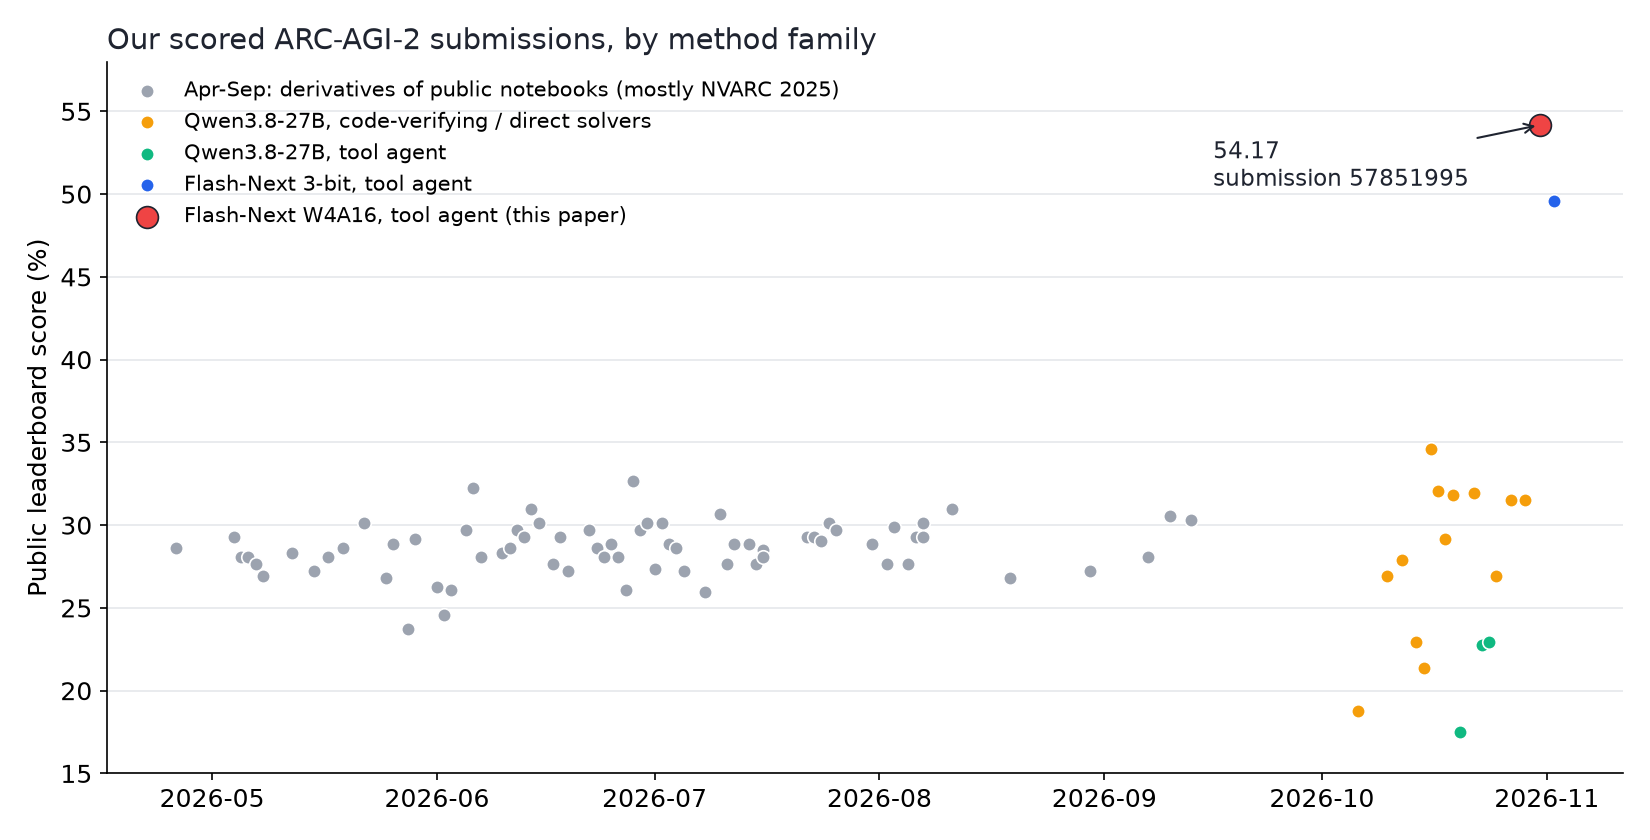
\includegraphics[width=\linewidth]{figures/fig2_lb_history.png}
\caption{Public leaderboard scores of our team's scored submissions (runs below 5 omitted). Repeated runs of one notebook vary by about $\pm$1.5 points.}
\label{fig:lb}
\end{figure}

\paragraph{April--September: test-time training.} About 70 submissions built on public notebooks, mostly of the NVARC 2025 lineage, scored 23.75--32.64. Our companion paper \cite{paper1} shows that in two logged evaluation runs 116--117 of 172 test inputs had no correct candidate above the search threshold, while perfect selection could add 4.67--7.67 points.

\paragraph{October: Qwen3.8-27B with code verification.} A Poetiq-style solver that writes code and checks it on the training pairs reached 34.58 with 60k thinking tokens per attempt. The same solver family with a 77.8k cap scored 48.61\,\% on the evaluation set but 21.39 on the leaderboard, and a 49k cap gave 32.08. A replay simulation of our logs estimated that about 208 of 240 hidden tasks receive a first iteration at 60k against about 177 at 77.8k. These notebooks differ in more than the cap, so we read the 13-point gap as consistent with lost coverage, not as a controlled result.

\paragraph{October: Qwen3.8-27B as a tool agent.} A Duck-style agent on the same model scored 17.50--22.92, below the code-verifying solver. In our first agent runs (per-response cap 49k) the first call to the checker came at a median of about 55k tokens; in later 120-task runs it came at 25--31k, still most of an attempt budget of 35--45k. The dense model reasoned at length before testing anything.

\paragraph{November: Qwen3.8-Flash-Next.} The same agent on the sparse model scored 54.17 (W4A16, this submission) and 49.58 (3-bit ``klee100'' build).

\section{System}\label{sec:system}
\begin{figure}[t]
\centering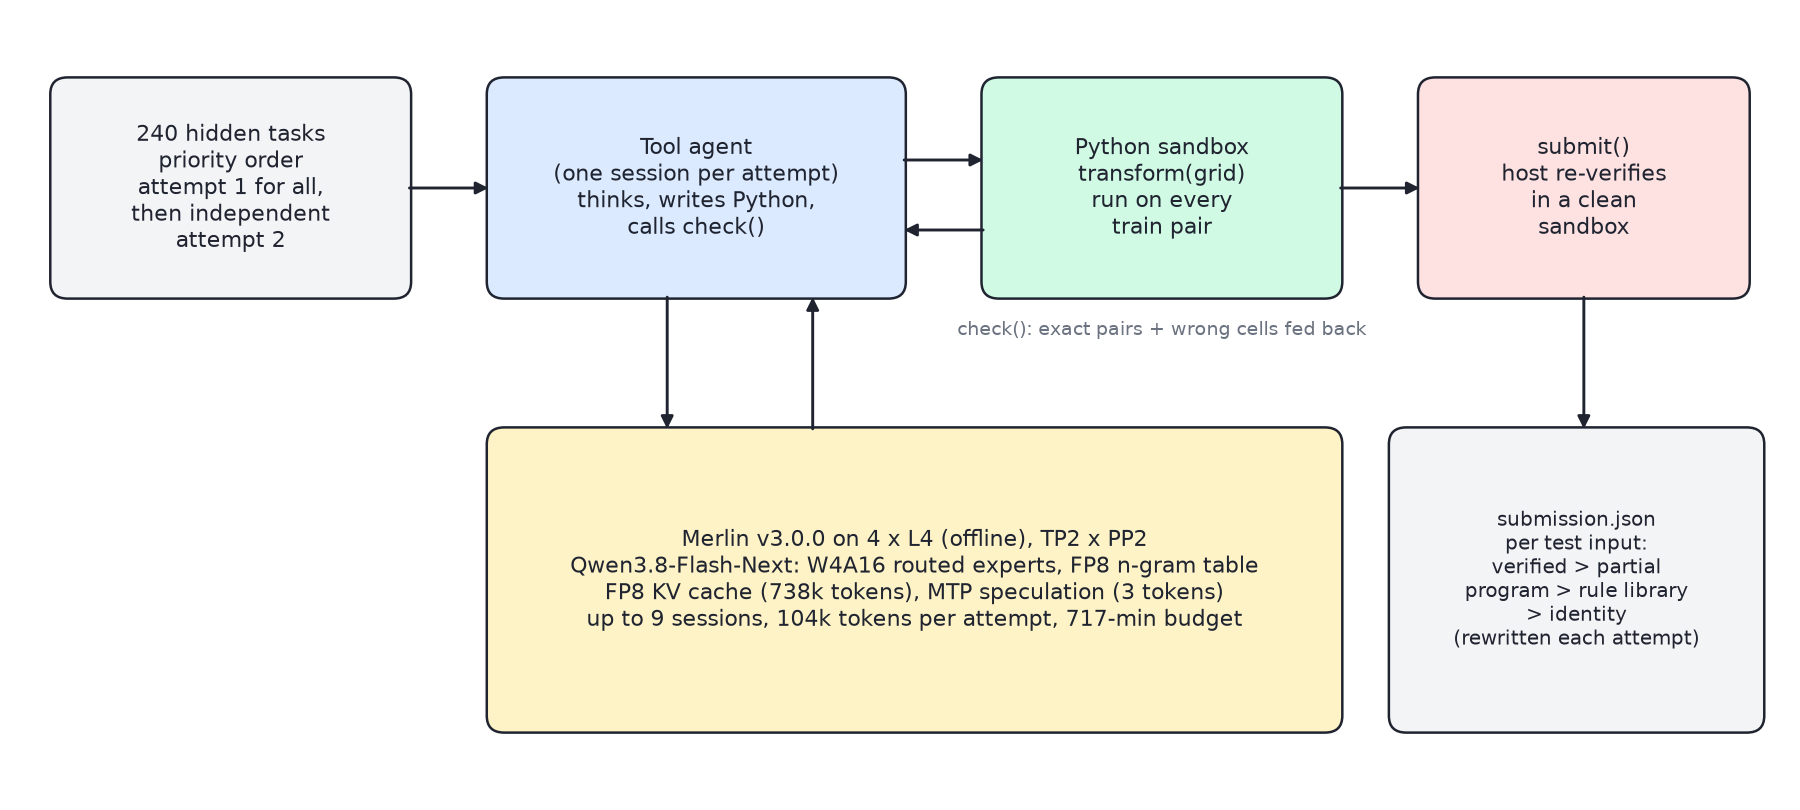
\includegraphics[width=\linewidth]{figures/fig1_pipeline.png}
\caption{Pipeline of submission 57851995. Details in Appendix~\ref{app:spec}.}
\label{fig:pipe}
\end{figure}

\paragraph{Model and engine.} Qwen3.8-Flash-Next \cite{qwen38} is a 48-layer mixture-of-experts model with 512 routed experts per layer, top-10 routing, multi-token-prediction heads and a large n-gram embedding table. We serve it with Merlin v3.0.0 \cite{merlin}, a vLLM-0.32 fork \cite{vllm}, using a W4A16 checkpoint (routed experts in 4 bits), an FP8 copy of the n-gram embedding table, an FP8 E4M3 KV cache (pool 738{,}142 tokens), tensor parallelism 2 $\times$ pipeline parallelism 2 with expert parallelism, prefix caching, and MTP speculation with 3 draft tokens and probabilistic acceptance (median accept length 2.88). If the engine fails to boot, the KV cache size steps down (at most three tries). Up to nine agent sessions run at once.

\paragraph{Agent.} Each attempt is one session with a single \texttt{python} tool in a sandbox (30\,s per call, 4\,GB address space). Raw grids are never in the prompt: the model sees a compact ``facts'' view (shapes, colour counts, changed cells, components) and reads exact grids inside Python. The loop is: reason, write \texttt{transform(grid)}, call \texttt{check()} (exact pairs, and up to six wrong cells per failing pair), revise, and call \texttt{submit()}, which the host re-verifies in a clean sandbox. Sampling: temperature 1.0, top-$p$ 0.95, top-$k$ 20, reasoning effort xhigh, 104k tokens per attempt.

\paragraph{Scheduling and answers.} Attempt~1 runs for every task first, in a priority order (tasks with at least three training pairs and a single test input first, then smaller grids). Attempt~2 is an independent session. Each test input is filled separately: train-verified programs first (agreeing candidates before single ones), then partially fitting programs, then a small rule library, then the test input itself. A complete \texttt{submission.json} with an identity fallback is written at notebook start and rewritten after every finished attempt, so unverified outputs are submitted when nothing verifies.

\section{Results}
\subsection{Leaderboard}
\begin{table}[h]
\centering\small
\begin{tabular}{@{}lr@{}}
\toprule
Method family (best submission) & Public LB (\%) \\
\midrule
NVARC-lineage test-time training & 32.64 \\
Qwen3.8-27B, code-verifying solver (60k) & 34.58 \\
Qwen3.8-27B, tool agent & 22.92 \\
Flash-Next 3-bit (klee100), tool agent (57896498) & 49.58 \\
\textbf{Flash-Next W4A16, tool agent (57851995)} & \textbf{54.17} \\
\bottomrule
\end{tabular}
\caption{Best public leaderboard score per family; one run each, noise about $\pm$1.5.}
\label{tab:lb}
\end{table}

\subsection{Precision of verification}\label{sec:precision}
We re-scored every train-verified program against the gold outputs, counting an attempt correct only if every test output matches.
\begin{table}[h]
\centering\small
\begin{tabular}{@{}llrrrl@{}}
\toprule
Sample & Build & Verified & Correct & Precision (95\,\% CI) & Fisher $p$ \\
\midrule
120 tasks, 6 h, attempt 1 & W4A16 & 79 & 61 & 77.2\,\% (66.8--85.1) & 0.037 \\
 & 3-bit & 104 & 65 & 62.5\,\% (52.9--71.2) & \\
15 matched tasks, 2 attempts & W4A16 & 26 & 24 & 92.3\,\% (75.9--97.9) & 0.25 \\
 & 3-bit & 28 & 22 & 78.6\,\% (60.5--89.8) & \\
3-bit, all 30 tasks & 3-bit & 54 & 41 & 75.9\,\% (63.1--85.4) & \\
\bottomrule
\end{tabular}
\caption{Share of train-verified programs that are correct on the test (Wilson intervals). The 6-hour builds differ from the submitted one (Section~\ref{sec:six}).}
\label{tab:prec}
\end{table}
In every sample the 3-bit build's verified programs were wrong more often (Table~\ref{tab:prec}, Figure~\ref{fig:ver}); the difference is significant on the largest sample. The direction agrees with notnitsuj's report \cite{notnitsuj2026}. On the 15 matched tasks the 3-bit build also spent 1.44$\times$ the tokens, and 34.5\,\% of its tokens went to attempts that verified but were wrong (W4A16: 18.1\,\%).

\begin{figure}[t]
\centering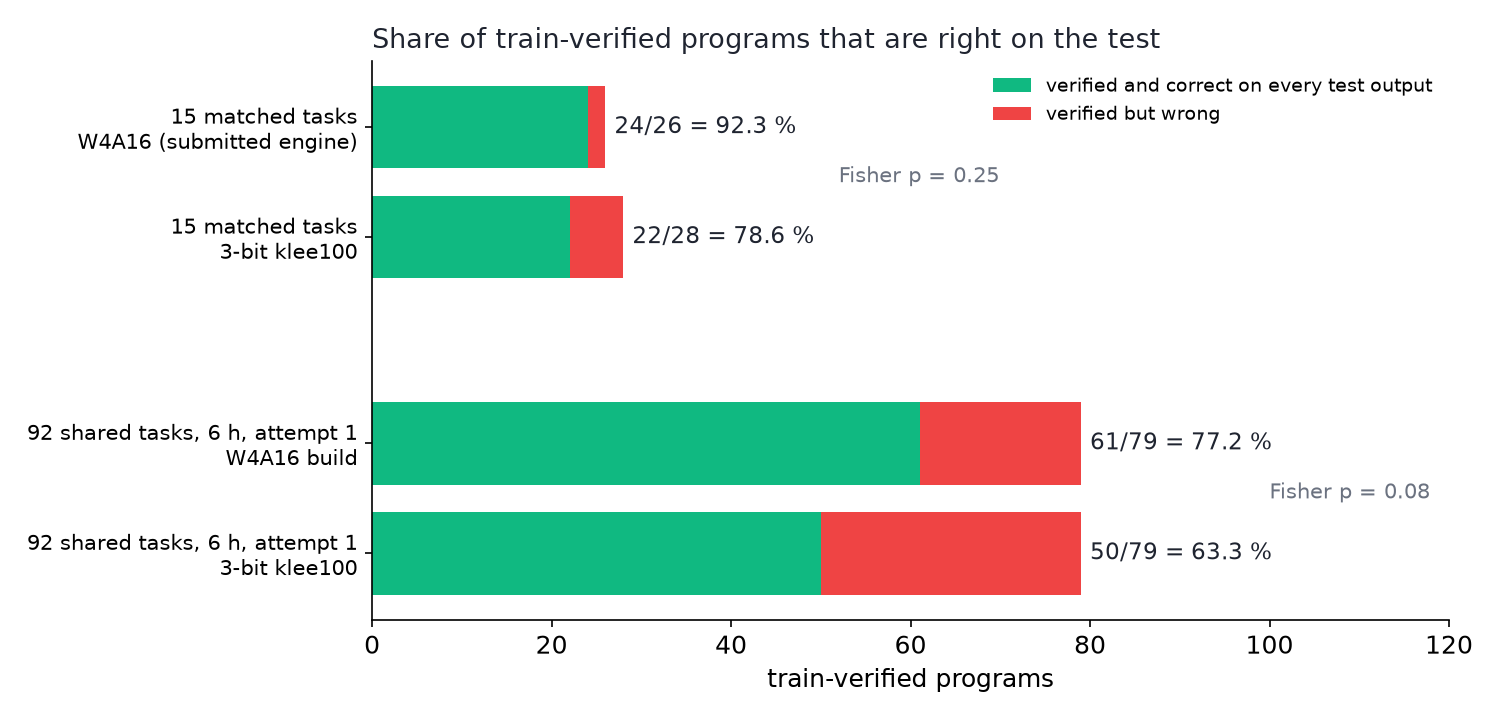
\includegraphics[width=0.85\linewidth]{figures/fig3_verification.png}
\caption{Train-verified submitted attempts, correct on every test output (green) or not (red).}
\label{fig:ver}
\end{figure}

\begin{table}[t]
\centering\small
\begin{tabularx}{\linewidth}{@{}lXr@{}}
\toprule
Class & Description (example) & Count \\
\midrule
(b) underdetermined rule & another rule fits all demonstrations but not the test (overlap priority of pasted shapes in 247ef758; cavity choice in 16b78196, two pairs) & 11 \\
(a) hard-coded structure & fixed column offsets or per-row caps tuned to the pairs; flagged by the agent's own \texttt{fixed\_offset} check but not blocked & 2 \\
(c) test outside demonstrations & 4$\times$4 test grid with a new colour; all pairs 8$\times$8 or 16$\times$16 & 1 \\
(d) output size & size from fitted arithmetic, wrong on larger test grids & 1 \\
\bottomrule
\end{tabularx}
\caption{All 15 train-verified wrong programs in the matched runs (13 from the 3-bit build, 2 from W4A16; both W4A16 cases are class (b) and produce the same wrong grids as the 3-bit build).}
\label{tab:fv}
\end{table}
Table~\ref{tab:fv} classifies all false verifications by reading the final program, the demonstrations and the gold output. Eleven are rules the demonstrations do not pin down. Nine of the thirteen 3-bit cases are wrong in at most 8 cells, and in seven the test grid is larger than every demonstration. The two W4A16 errors are byte-identical to 3-bit errors, so on those tasks the cause is the task's ambiguity, not quantization.

\subsection{Memory and concurrency}
In a paired run on the same 15 tasks (same seed, equal 4{,}050\,s windows), FP8 and BF16 KV caches each solved 13 tasks (18/20 outputs; task-normalised 86.67 vs 90.00; McNemar $p=1.0$, 2 discordant tasks). FP8 gave 1.9$\times$ the KV pool (214 vs 112 blocks), 9 sessions instead of 5, and raised the steady decode median from 169 to 225 tok/s. Nine sessions of up to 104k tokens need far less than $9\times104$k of live KV: the peak live context was 363{,}807 tokens (49\,\% of the pool) over 5 requests, with no preemption and only 3 of 270 requests queued, all in the first 50\,s.

\subsection{Coverage versus precision at six hours}\label{sec:six}
Both builds ran the 120 public evaluation tasks in 6-hour windows (Table~\ref{tab:six}). These builds are not the submitted ones: the W4A16 run used 12 sessions, alphabetical order, a scheduler with re-runs and an int8 draft head; it was KV-starved (2{,}028 preemptions). The 3-bit run (24 sessions) is the build submitted as 57896498.
\begin{table}[h]
\centering\small
\begin{tabular}{@{}lrrrrr@{}}
\toprule
Build (6 h, 120 tasks) & tok/s & Tokens & Tasks started & Outputs /172 & Task-norm.\ \% \\
\midrule
W4A16, 12 sessions & 182.3 & 3.94\,M & 92 & 90 & 53.75 \\
3-bit klee100, 24 sessions & 419.4 & 9.06\,M & 120 & 107 & 65.00 \\
\bottomrule
\end{tabular}
\caption{Six-hour evaluation runs.}
\label{tab:six}
\end{table}
The decomposition is clean. On the 92 tasks both builds reached, W4A16 solved 63 and the 3-bit build 57; at equal token spend (3.0\,M) W4A16 had solved 44 tasks and the 3-bit build 32. The 3-bit build's lead on evaluation comes entirely from the 28 tasks W4A16 never started, of which it solved 17. The W4A16 build was still gaining 15 tasks in its last hour.
On the hidden set, the submitted W4A16 build runs 9 uncontended sessions instead of 12 starved ones, so it reaches further at the same time per task; there the higher precision paid off (54.17 vs 49.58, one run each).

\subsection{Evaluation as a proxy for the leaderboard}
Three inversions: (1)~the 3-bit build beat a W4A16 build on evaluation (65.00 vs 53.75 task-normalised) and lost on the leaderboard; (2)~our 27B solver at a 77.8k cap scored 48.61\,\% on evaluation and 21.39 on the leaderboard, below its 60k version; (3)~we ran two public Flash-Next notebooks by other teams on the evaluation set under equal 5\,h\,23\,min windows: nisshokuitsuki's \cite{ni2026} answered 151/172 outputs and Domdolus's \cite{domdolus2026} 139/172, while their published leaderboard scores are in the opposite order (77.22--78.06 vs 83.47). Candidate reasons are the per-task budget of evaluation runs, the different difficulty of the hidden set, and use of public evaluation tasks in training; we did not test them.

\section{Why it works}
\paragraph{The demonstrations are a unit test of varying strength.} A program that reproduces every demonstration encodes some rule that explains them; whether it is the intended rule depends on how many alternatives the demonstrations leave open. With two or three pairs, or a test grid larger than all of them, several programs fit, and Table~\ref{tab:fv} shows that false verification lives there. A stronger model is more likely to pick the simplest rule a person would pick; the 3-bit model, which also spent 44\,\% more tokens per task, more often settled on a rule that fits but was not intended.

\paragraph{Coverage and precision trade against each other.} The score is approximately $\sum_{\text{tasks}} P(\text{reached})\,P(\text{verified}\mid\text{reached})\,P(\text{correct}\mid\text{verified})$ plus unverified fallbacks. Section~\ref{sec:six} measures the first and third factors separately: the faster build raised the first and lowered the third. Which effect wins depends on how many tasks the slower build reaches anyway. On the hidden set, 717 minutes at 172--225 tok/s give about 8.8\,M tokens after a 13--17 minute boot, roughly 37k per task. In our 15-task run, correct first attempts needed a median of 6.3k tokens on usually-solved tasks and 23.6k on sometimes-solved ones, so this budget reaches most solvable tasks without extra speed, and precision decides the rest.

\paragraph{Memory sets concurrency.} An L4 has 24\,GB. 4-bit experts make the model fit; the FP8 KV cache doubles the sessions that fit next to it without measured loss. Too many sessions for the pool cause preemption and lose more than they gain (Section~\ref{sec:six}).

\paragraph{Second attempts are cheap insurance in our regime.} With W4A16 on 15 tasks, attempt~2 rescued one test output (247ef758) in a task where attempt~1 had a verified but partly wrong program; with the 3-bit build, second attempts after a verified first attempt used 45\,\% of its tokens and rescued none. Public systems with more throughput report larger gains from independent sessions and voting \cite{majkel2026,yichia2026}.

\section{What did not work, and a path forward}\label{sec:progress}
\paragraph{Negative results} (27B runs unless noted):
\begin{itemize}
\item \emph{Early stopping} of hopeless attempts: the best text signal reached AUC 0.61--0.64, saved 2.7--4.0\,\% of tokens, and out of sample lost 18\,\% of train-passing attempts (consistent with \cite{notnitsuj2026}).
\item \emph{Pause and resume} at 30--60k tokens was worse than a straight run at every budget.
\item \emph{Thinking caps} of 49k and 77.8k scored below 60k on the leaderboard (32.08 and 21.39 vs 34.58), in separate notebooks.
\item \emph{Task ordering} by difficulty predicted from the task file did not beat a simple priority order, which beat random order by 3.7--6.8 points at 50--70\,\% budgets in a replay simulation.
\item \emph{A dense 27B tool agent} scored below the same model with a code-verifying solver.
\item \emph{A faster 3-bit Flash-Next build} and \emph{12 sessions on a pool sized for 9} both lost to the slower, uncontended W4A16 configuration.
\end{itemize}

\paragraph{Headroom from complementary systems.} On the 120 public evaluation tasks our best single run answered 107 of 172 test outputs and the union of all our runs up to the deadline answered 143 (task-normalised 85.69\,\%). Adding the two public notebooks above gives 161 of 172 (95.28\,\%); 11 outputs in 8 tasks were answered by none. This is an oracle over many runs, not a reachable score, but it shows that systems fail on different tasks.

\paragraph{Next steps, with public evidence.}
\begin{enumerate}
\item \emph{Acceptance test:} measure verified precision on a fixed task set before shipping any compression or concurrency change.
\item \emph{Targeting class (b):} invariants and symmetry tie-breaks (+2.6 and +0.54 points reported by \cite{notnitsuj2026}), rejecting hard-coded structure (our own \texttt{fixed\_offset} flag caught both class-(a) cases but did not block them; see also \cite{majkel2026}), and induced-rule checks \cite{ni2026}.
\item \emph{Skip duplicate second attempts:} 3-bit second attempts after an already-correct first attempt used 598k tokens in the 6-hour run.
\item \emph{Portfolio:} route tasks without a verified program to a different solver, using the union headroom above.
\end{enumerate}

\section{Universality and limitations}
\paragraph{A general rule.} For any execute-and-check agent on fixed hardware (code generation with unit tests, programming by example, data-wrangling scripts, proof search with a checker), the verifier's pass rate is not its precision. Accept a compression or speed change only if verified-answer precision times verified answers per hour does not fall; tokens per second and teacher-forced divergence do not measure this. The rule cannot protect against errors the verifier cannot see, which in ARC is the underdetermined-rule class (b); there, more demonstrations or a second, independent check are needed.
\paragraph{Limitations.}
\begin{itemize}
\item Leaderboard comparisons rest on one run per build (noise about $\pm$1.5 points); the submitted build was not run on all 120 evaluation tasks.
\item The precision difference is significant only on the largest sample; the 6-hour builds differ from the submitted ones.
\item Qwen3.8 models may have seen public ARC data in training; we cannot measure this.
\end{itemize}

\section{Conclusion}
A Qwen3.8-Flash-Next tool agent with 4-bit routed experts, an FP8 KV cache and speculation on four L4 GPUs scored 54.17 on the ARC-AGI-2 public leaderboard, about 20 points above our dense-model and test-time-training systems. A faster 3-bit build covered more tasks but verified wrong rules more often, mostly where the demonstrations leave the rule open, and scored lower on the leaderboard. For systems that grade their own answers, verified-answer precision belongs next to tokens per second in every engineering decision.

\section*{Reproducibility and artifacts}
Public notebook of the submission: \url{https://www.kaggle.com/code/foysalemonshanto/q27-xhigh-e25-nb6-submit} (version~1, submission~57851995). Engine: Merlin v3.0.0 (\url{https://github.com/halt95/merlin-engine}, commit \texttt{ad42e37f}). Papers, figures and analysis scripts: \url{https://www.kaggle.com/datasets/foysalemonshanto/arc2026-hack2publish-papers}.

\section*{Use of AI tools}
AI coding and writing assistants were used to write analysis scripts and draft text. All numbers were taken from saved run outputs and checked against them.

\bibliographystyle{plain}
\bibliography{refs}

\appendix
% Appendix: agent and engine specification of submission 57851995
% (notebook foysalemonshanto/q27-xhigh-e25-nb6-submit v1; hidden-rerun profile RERUN_PROD).
% Every item is taken from the notebook code and the agent payload; file:line evidence in appendix_spec_EVIDENCE.md.
\section{Agent and engine specification}\label{app:spec}
\sloppy\raggedright

This appendix lists the configuration that the hidden rerun of submission 57851995 executes (profile \texttt{RERUN\_PROD}). The agent is the Duck tool-agent harness of Tufa Labs as forked by D.~Franzen (\texttt{da-fr/arc-agi-3-solution} at commit \texttt{10882e33}, Apache-2.0), vendored byte-identical except for two switched-off-by-default patches, plus our ARC-AGI-2 adapter \texttt{arc2\_duck.py}. Both ship in the payload dataset \texttt{q27-e15b-payload} and are verified by SHA-256 before use. The served model name is \texttt{q27}; the weights are Qwen3.8-Flash-Next.

\subsection{Prompt and task representation}
The system prompt holds the task; the first user turn is a short opener. Excerpt of the system prompt (elisions marked):
\begin{quote}\small
``You are a Python coding agent solving an ARC-AGI-2 grid task. [\dots] The training pairs show one transformation from input grid to output grid. Infer it and implement it as a top-level function \texttt{transform(grid)} that takes and returns a rectangular list of lists of ints 0-9. It is then applied to each test input; the test outputs are unknown to everyone. [\dots] The exact grids are not repeated in this prompt. They are in the python tool as \texttt{train} [\dots] and \texttt{test\_inputs} [\dots]. The facts below were computed from them by the harness: observations, not a rule [\dots]. A train-exact function is not proof that it generalizes. \texttt{submit(transform)} submits your final choice and ends this branch; submit only a function that check shows exact.''
\end{quote}
\begin{itemize}[leftmargin=*,itemsep=1pt]
\item \textbf{Grids are not printed in the prompt} (view \texttt{facts} for both attempts). The prompt carries a ``facts'' block computed from the exact grids: per training pair the input/output shape, colour counts, modal colour, changed-cell count and bounding box (same-shape pairs) or the shape change, connected-component counts and the largest components; per test input the shape, colours and components. The block is bounded to 800 tokens and 3{,}600 characters by dropping detail levels, and says what was dropped.
\item The exact grids are Python lists in the sandbox (\texttt{train}, \texttt{test\_inputs}). \texttt{show(g, r0, c0, r1, c1)} prints an indexed view (\texttt{r03 | 0 0 5 \dots}), at most 900 cells per view and 1{,}000 per call; raw grid-row prints in tool output are cut by the harness.
\item The prompt also states the token budget of the attempt (``about 104,000 generated tokens, thinking included''), the allowed imports (no numpy), the 30-s tool time limit and the tool-output cap.
\end{itemize}

\subsection{Tools}
The model has exactly one tool, \texttt{python} (a persistent sandbox; top-level functions are retained across calls). Inside it the harness provides:
\begin{itemize}[leftmargin=*,itemsep=1pt]
\item \texttt{check(transform, verbose=True)}: runs \texttt{transform} on every training pair and once on each test input. It prints \texttt{check(name): k/n train pairs exact; test inputs: ok, \dots} (plus an identity flag), then for each failing pair the error with its line, or the shape mismatch, or the wrong-cell count with up to 6 samples \texttt{(row, col, got, expected)}. It returns a list of per-pair dicts (\texttt{ok}, \texttt{wrong\_cells}, samples, or \texttt{error} / \texttt{shape}). A train-exact result is reported to the host, which re-runs the function in a clean sandbox and, if exact, keeps it as a candidate answer; the attempt continues.
\item \texttt{check\_many(\{label: f, \dots\})}: the same for several functions.
\item \texttt{submit(transform)}: needs a named top-level function. The host re-runs it in a clean sandbox, one sandbox per grid, with only the retained sources and one input grid, reads the value from the sandbox's structured result, and compares it with every training output. Accepted (exact on all pairs and valid test outputs) ends the attempt; otherwise the rejection summary is returned and the attempt continues.
\item Exploration helpers: \texttt{arc\_overview}, \texttt{inspect\_pair}, \texttt{inspect\_test}, \texttt{show}. Grid functions usable inside \texttt{transform}: \texttt{grid\_shape}, \texttt{color\_counts}, \texttt{modal\_color}, \texttt{components}, \texttt{bbox}, \texttt{crop}, \texttt{rot90}, \texttt{flip\_h}, \texttt{flip\_v}, \texttt{transpose}, \texttt{diff\_cells}, \texttt{diff\_summary}, \texttt{object\_diff}.
\item Auto-check: after a call that defines a one-grid function named \texttt{transform*}, \texttt{solve*}, \texttt{candidate*}, \texttt{trans}, \texttt{trans\_*} or \texttt{*\_alt}, the harness checks it (at most 3 per call, 24 per attempt; at most 24 host verifications of exact \texttt{check} results per attempt). \texttt{submit}/\texttt{check} sent as tool names are run as Python.
\end{itemize}

\subsection{Sampling and limits}
{\small
\begin{longtable}{@{}>{\raggedright\arraybackslash}p{0.36\linewidth}>{\raggedright\arraybackslash}p{0.58\linewidth}@{}}
\toprule
Item & Value \\
\midrule
Temperature / top-$p$ / top-$k$ & 1.0 / 0.95 / 20 (per request; the server's generation override is the same, with min-$p$ 0, presence 0, repetition 1.0) \\
Seed & none sent \\
Thinking & on; \texttt{reasoning\_effort = xhigh} per request and as the server's chat-template default \\
Attempt budget & 104{,}000 generated tokens (attempt 1 and attempt 2), thinking included; a 60{,}000-token thinking floor is asserted \\
Output per request & remaining budget $-$ 4{,}096 (reserve); further clamped to $120{,}384 - \text{prompt} - 2{,}048$ (120{,}384 = 8{,}192 prompt + 104{,}000 + 8{,}192 tool allowance) \\
Commit turn & when $\le$ 5{,}120 tokens remain, the harness asks for one final \texttt{transform} + \texttt{check} call; it is an ordinary thinking-on request (``variant A'') \\
Context & server max-model-len 131{,}072; agent window 130{,}560; raw reasoning kept in history \\
Request timeout & 3{,}600 s, clamped to the solve deadline \\
Tool steps / turns & no step cap (\path{LOCAL_ANALYZER_TOOL_STEPS = 0}); an attempt ends on acceptance, budget, deadline or repeated failures \\
Sandbox & 30 s per call (CPU limit 31 s), address space 4{,}096 MB (\texttt{RLIMIT\_AS}, read back per child; not verified $\Rightarrow$ solver disabled), file size 1 MB, 32 open files, standard-library subset only \\
Tool output & capped to about 3{,}072 tokens \\
\bottomrule
\end{longtable}}

\subsection{Attempt policy and answer selection}
\begin{itemize}[leftmargin=*,itemsep=1pt]
\item Two independent attempts per task (fresh agent, new conversation each), both 104{,}000 tokens, both with the facts view. No pause or resume, no third attempt (\texttt{extra\_attempts} off); attempt~2 is not skipped when attempt~1 verified, it only needs time left.
\item Stage 1: attempt~1 of \emph{every} task, in the task order below. Stage 2: attempt~2, queued when attempt~1 of that task ends, ranked by evidence class: 0 = partial progress but no verified program, 1 = nothing, 2 = one distinct verified prediction, 3 = two or more. Accepts made after the commit text (``weak'') do not count toward the class.
\item End of an attempt without a verified program: (1) functions written only in the reasoning or text are extracted, run and checked (an exact one goes through host verification); (2) the best partial function (most exact training pairs, then changed-cell accuracy) is host-run once on train and test; its test output is kept as a \emph{non-accepted} candidate.
\item Selection, per test input: each attempt's best (latest accepted \texttt{submit}, else latest accepted \texttt{check}) is grouped by identical output; groups are ordered by (contains a non-weak accept, number of attempts agreeing, explicit submission, earlier attempt, latest). Then other accepted candidates (latest first), then non-accepted partial candidates (most exact pairs, then latest), then outputs of a small CPU rule library (rotations, flips, transposes, crop, scales, tilings, mirrors, a global colour map) that are exact on every training pair. \texttt{attempt\_1} = first grid; \texttt{attempt\_2} = next distinct grid, else the test input.
\item So an \emph{unverified} answer is submitted when no attempt verifies: the best partial program's output.
\item Fallback: the test input itself (identity) for both attempts, written for every task at notebook start; a task whose selection fails also falls back to identity.
\item Tasks with several test inputs: one \texttt{\{attempt\_1, attempt\_2\}} per test input, each selected independently from the same programs.
\end{itemize}

\subsection{Task order (ORDER2)}
Tasks are sorted by $-(\,[\#\text{train pairs}\ge 3] + [\#\text{test inputs} = 1]\,)$, then by the total number of cells (train inputs + outputs + test inputs) ascending, then by task id. Attempt~1 of all tasks follows this order.

\subsection{Engine}
\begin{itemize}[leftmargin=*,itemsep=1pt]
\item \textbf{Merlin} v3.0.0, a public vLLM 0.32.0 fork (\path{github.com/halt95/merlin-engine}, tag \texttt{merlin-v3.0.0}, commit \texttt{ad42e37f}, wheel \path{vllm-0.32.0+merlin.7002f56537}). It is installed offline in the notebook from our Kaggle Model \texttt{e23-merlin-env} (\texttt{install\_merlin\_offline.sh}); the server command comes from Merlin's own \texttt{launch.build("flash-next", "fn-quad-24g-sm89", \dots)}.
\item \textbf{Weights}: five W4A16 checkpoint parts (Kaggle Models \path{qwen3-8-flash-next-w4a16-merlin-p1..p5}) and an FP8 n-gram embedding table (PLE) overlay, merged by symlink with size checks (the rerun has no SHA gate).
\item \textbf{Layout}: 4$\times$L4, tensor parallel 2 $\times$ pipeline parallel 2 with expert parallelism; block size 4{,}096; max-num-batched-tokens 1{,}024; GPU memory utilisation 0.96.
\item \textbf{KV}: FP8 E4M3 with static QSA scales (\texttt{qsa\_kv\_scales\_262k.json}). \textbf{Pin ladder}: \texttt{-{}-kv-cache-memory-bytes} = Merlin's L4 pin 2{,}479{,}838{,}700 B + 1.0 GiB = 3{,}553{,}580{,}524 B first, then +0.75 / +0.5 / +0 GiB. The ladder starts at +1.0 only if the \#60490 patch verified, else at +0.
\item \textbf{\#60490}: a backport of vLLM PR \#60490 (issue \#60489) into Merlin's \texttt{qsa.py}: during the memory-profiling dummy run the QSA indexer allocates its peak scratch (max of the prefill logits budget and decode tokens $\times$ compressed columns $\times$ 4 B, plus the top-$k$ workspace), so the profiler accounts for it. Applied with pinned pre/post SHA-256.
\item \textbf{Speculation}: MTP, 3 draft tokens, \path{draft_sample_method = probabilistic}; the boot read-back checks method \texttt{mtp} and $K=3$.
\item \textbf{Prefix caching} on (\texttt{-{}-enable-prefix-caching}, \texttt{-{}-mamba-cache-mode align}, \texttt{-{}-prefix-match-unit 64}); \texttt{-{}-use-replayssm}.
\item \textbf{CAPS16}: \path{cudagraph_mode} \path{FULL_AND_PIECEWISE} with capture sizes 1, 2, 3, 4, 6, 8, 12, 16, 24, 32, 40, 48, 64 (FULL decode graphs cover 16 $\times$ (1+3) tokens).
\item \path{MERLIN_SHARE_DRAFT_WORKSPACE=1}: Merlin environment switch, in the plan described as the MTP draft sharing the target's workspace; dropped automatically if an error line names it or every pin step fails with it.
\item \textbf{Measured F}: $F = \lceil F_{\log} - 0.05\rceil$ with $F_{\log} = \text{pool}/X - \lceil M/B\rceil$ from the server's own ``Maximum concurrency for $M$ tokens per request: $X$x'' line (fixed blocks per request).
\item \textbf{Concurrency}: workers $=\min\big(\lfloor \text{pool}/(\lceil 65{,}536/B\rceil + F)\rfloor,\ \texttt{max-num-seqs}\big)$, with \texttt{-{}-max-num-seqs} 9 / 8 / 8 / 6 on the four pin steps; the production boot therefore runs up to 9 agent sessions. If the pre-solve isolation check is not PASS, workers drop to 6.
\item \textbf{Slots admission}: an attempt starts when one of the \emph{workers} slots is free (the engine schedules KV; preemptions are allowed and counted); an attempt whose projected peak exceeds the whole pool never starts. The scheduler's KV gate is set to 1.0. No new attempt starts with less than 300 s to the solve end.
\end{itemize}

\subsection{Run safety}
\begin{itemize}[leftmargin=*,itemsep=1pt]
\item Clock anchored at kernel start. Budget 12\,h $-$ 3\,min = 717 min; hard stop at 715 min; solving ends 180 s before it (712 min), every request clamped to that deadline, then a 90-s join grace; the engine cell's watchdog kills live servers at 717 min.
\item No separate drain: the drain and admit deadlines of the time block are defined but not used on this path; the per-attempt budget, the deadline clamp and the 300-s admission cutoff end the work.
\item Boot ladder: at most 3 engine attempts (30, 15, 15 min ready timeouts); ready = \texttt{/health} answers and the server log shows its KV-cache line; 600 s of log silence = stall; any failure before solving moves to the next pin step; no new try with less than 25 min left.
\item Server watchdog during solving (10-s poll): a dead process, a silent log with \texttt{/health} failing for 180 s, or 600 s without token progress while requests run triggers a relaunch with the same plan (at most 2 watchdog actions, only with $\ge$ 20 min left, and $\ge$ 35 min before the solve end; ready wait $\le$ 20 min; a sampled check must pass). Attempts wait while the server is down.
\item Submission: the identity \texttt{submission.json} is written at the start; it is rewritten atomically after every finished attempt (until the solve end) and once more at the end.
\item The sandbox self-test and the memory-limit test must pass, else the solver does not run and the identity file stays.
\end{itemize}

\subsection{The 3-bit ``klee100'' build (submission 57896498)}
Notebook \path{esfersami50/q27-xhigh-e28-k100-eval120-6h}. Its \texttt{RERUN\_PROD} is the profile above plus the E28 levers; everything not listed (12\,h $-$ 3\,min budget, boot ladder, slots admission, measured F, \#60490, shared draft workspace, MTP $K=3$ probabilistic, max-model-len 131{,}072, prompt, tools, sampling) is the same.
{\small
\begin{longtable}{@{}>{\raggedright\arraybackslash}p{0.2\linewidth}>{\raggedright\arraybackslash}p{0.36\linewidth}>{\raggedright\arraybackslash}p{0.36\linewidth}@{}}
\toprule
 & W4A16 (57851995) & klee100 (57896498) \\
\midrule
Routed experts & W4A16 (5 parts) & AutoRound 3bpw-MTP (\path{klee100/Qwen3.8-Flash-Next-AutoRound-3bpw-MTP}): W3 g128 on layers 0--11 and 36--47, W2 g64 on 12--35 (humming kernels); MTP experts W4; main projections W8 \\
KV scales & W4 checkpoint's QSA sidecar & the same W4 sidecar reused (labelled experimental) \\
Extra flags & -- & \texttt{-{}-language-model-only}, a read-only worker extension \\
Pin ladder (KV bytes) & 3.55 / 3.29 / 3.02 / 2.48 GB & 7.93 / 6.86 / 5.27 / 3.55 / 2.48 GB \\
Workers & up to 9 & 24 on the top rung (\texttt{-{}-max-num-seqs 24}); lower rungs $\min(\text{rule}, 18 / 14 / 9 / 6)$ \\
CUDA graphs & CAPS16 (to 64) & sizes to 84 \\
Q-defer & off & on when its patch verifies (\texttt{NB4\_PPDEFER=1}): the pipeline stage-0 receive of sampled tokens is posted after the next forward launch \\
I8 & off & \texttt{DRAFT\_HEAD=int8} (int8 MTP draft LM head), kept only on read-back \texttt{I8\_ENGAGED} \\
C12 & off (9 workers) & not applicable (C12 = 12 streams, a W4 lever) \\
Request timeout & 3{,}600 s & 7{,}200 s (A/B1/C); 9{,}000 s (B2) \\
Thinking budget & 104{,}000 per attempt & A, B1, C: 104{,}000; B2: 120{,}000 \\
Order & ORDER2 & plain (sorted task ids) \\
Scheduler & attempt 1 for all, then attempt 2 & A: attempt 1 for all; B: re-run of attempt-1 failures (B1 = ended on its own without a full train match, same budget; B2 = cut by budget/context, 120k); C: attempt 2, first tasks still without a train match, then the rest by ascending attempt-1 tokens \\
Answer slots & selection above & \texttt{attempt\_1} = best-train candidate of A/B (a full-match B replaces A, the old A answer becomes the fallback); \texttt{attempt\_2} = C's candidate if different \\
\bottomrule
\end{longtable}}


\end{document}
